\chapter{Proposed approach: Building a graphic for visualizing unstructured data}
\label{chap_dev}
	
\section*{Introduction}

Data visualization is the process of displaying data/information in graphical charts, figures and bars. It is used as means to deliver visual reporting to users for the performance, operations or general statistics of an application, network, hardware or virtually any IT asset. \\

Data visualization is typically achieved by extracting data from the underlying IT system. This data is generally in the form of numbers, statistics and overall activity. The data is processed using data visualization software and is displayed on the system's dashboard. It is generally done to assist IT administrators in getting quick, visual and easy-to-understand insight into the performance of the underlying system. Most IT performance monitoring applications use data visualization techniques to provide statistical insight of performance of the monitored system.
\newpage




\section{Unstructured data}
Unstructured data represents any data that does not have a recognizable structure. It is unorganized and raw and can be non-textual or textual. For example, email is a fine illustration of unstructured textual data. It includes time, date, recipient and sender details and subject, etc., but an email body remains unstructured. Unstructured data also may be identified as loosely structured data, wherein the data sources include a structure, but not all data in a data set follow the same structure.
Unstructured data refers to data that follows a form that is less ordered than items like spreadsheet pages, database tables or other linear or ordered data sets. In fact, the term "data set" is helpful because it is associated with data that is in neat, accessible arrays, without any extra content, and that is linked or tagged in a specific structure. \\

Other instances of unstructured textual data include Word documents, PowerPoint presentations, instant messages, collaboration software, documents, books, social media posts and medical records. Non-textual unstructured data is generally created in media, such as MP3 audio files, JPEG images and Flash video files, etc. \\

Unstructured data usually does not include a predefined data model, and it may not match well with relational tables. Unstructured data is usually text heavy. However, it may include numbers and dates, as well as facts. This leads to ambiguities that are difficult to identify using conventional software programs. \\


The storage of huge volumes of unstructured data generated within an enterprise, if poorly managed, may lead to higher expenses. Data in hard copy documents or in an electronic format must be scanned in order for a search application to parse out ideas, depending on words used in certain contexts. This is known as enterprise or semantic search. \\

In customer-centered businesses, the data found in an unstructured form may be examined to enhance relationship marketing and customer relationship management (CRM). As social media apps, such as Facebook and Twitter, go mainstream, unstructured data development is likely to outrun the progress of structured data.  \\

\section{Proposed approach}
In order to accomplish the On demand graphical representation, our approach has essentially 3 steps to follow: Document analysis, Ontology construction, Document Annotation as shown in the figure \ref{fig_app}. We will enumerate and specify each of these main steps.  
%%description gènérale de l'approche  avec figure



\begin{figure}[H]
\centering
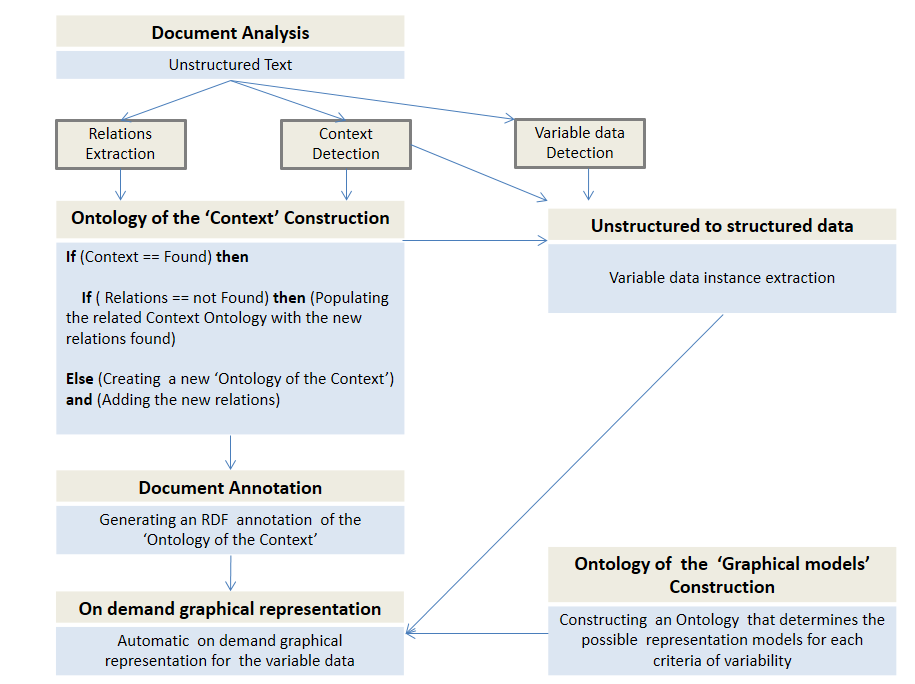
\includegraphics[scale=0.6]{plsfinal}
\caption{Execution flow of the on demand graphical representation}
\label{fig_app}
\end{figure}

\section{Document analysis}
\label{sec_anal}
%%Unstructured text analysis
Natural Language Processing (NLP) \cite{nlp} is a way for computers to analyze, understand, and derive meaning from human language in a smart and useful way. By utilizing NLP, developers can organize and structure knowledge to perform tasks such as automatic summarization, translation, named entity recognition, relationship extraction, sentiment analysis, speech recognition, and topic segmentation (see Figure \ref{fig_nlp}).

NLP is used to analyze text, allowing machines to understand how human’s speak. This human-computer interaction enables real-world applications like automatic text summarization, sentiment analysis, topic extraction, named entity recognition, parts-of-speech tagging, relationship extraction, stemming, and more. NLP is commonly used for text mining, machine translation, and automated question answering. 

NLP is characterized as a hard problem in computer science. Human language is rarely precise, or plainly spoken. To understand human language is to understand not only the words, but the concepts and how they’re linked together to create meaning. Despite language being one of the easiest things for humans to learn, the ambiguity of language is what makes natural language processing a difficult problem for computers to master. 

The figure \ref{fig_nlp} \cite{corenlp} below shows the overall system architecture of NLP.

\begin{figure}[H]
\centering
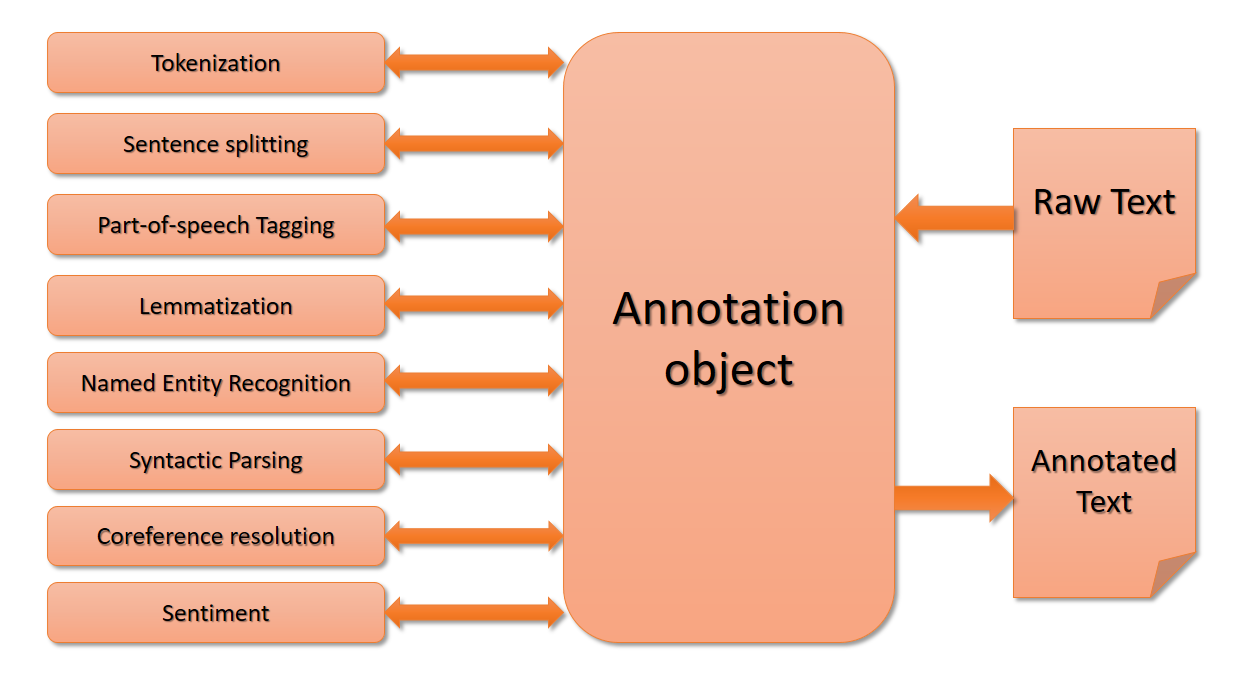
\includegraphics[scale=0.5]{nlpflow}
\caption{Overall system architecture of NLP}
\label{fig_nlp}
\end{figure}
\newpage

The process of analyzing a document can be categorized in four main steps: tagging, annotating, coreference and sentiment.

%%\renewcommand{\labelenumi}{\Roman{\enumiv}}
\begin{itemize}
   \item \textbf{Tagging\cite{corenlp}:} \\
   Tagging is a core task in Natural Language Processing. It consists in associating to each token a label providing certain information (e.g. syntactic category, number, verb tense…). Five main steps have been identified while tagging textual information: 
   \begin{itemize}
     \item \textbf{Sentences segmentation:} is the first step of the tagging process. A sentence can be defined as one or more words forming a syntactic unit. This segmentation allows dividing the text into its component sentences. 
     \item \textbf{Tokinization:} is the second step that allows identifying of the textual units that form the different sentences.
     \item \textbf{Tagging:} helps to classify words into their lexical categories and labeling them accordingly.
     \item \textbf{Lemmatization:} grants the representation of each word by its canonical form.
     \item \textbf{Syntactic parsing:} provides full syntactic analysis including through dependency representation between the words in order to identify the simple groups (nominal group, verbal group ...). 
   \end{itemize}
   \item \textbf{Named Entity Recognition:} \\
   Named Entity Recognition \cite{ner} labels sequences of words in a text which are the names of things, such as person and company names, or gene and protein names. It comes with well-engineered named entity recognizers for the English language. It particularly determines four classes (PERSON, ORGANIZATION, LOCATION, DATE).
   
   \item \textbf{Coreference resolution:} \\
   A Coreference is a relationship between two or more expressions in a text that refer to the same person or thing. The Coreference resolution \cite{corenlp} is the process in which we identify different reference chains. It is also known as Coreference in NLP techniques.
   
   \item \textbf{Sentiment:} \\
  Sentiment Analysis is the last method of NLP, it is a technique that is used to extract, identify, or otherwise characterize the sentiment content of a text unit. It is also known as "Opinion mining".

\end{itemize}

The first step in our proposed approach is analyzing an unstructured text document as an input data to detect the context related to that and to determine the variable data and statements using various NLP techniques \cite{maha}.   

We now present how to use these techniques to initially identify the context of a document, the named entities and the relations in-between them, and lastly, detecting the different variables that can be graphically plot. 



\subsection{Context detection}
\label{sec_21}

As the definition, a context is a part of a text or statement that surrounds a particular word or passage and determines its meaning. The context of a given document is identified from its main topics \cite{maha}. \\
The topics identification process can be acquired by obtaining the most important textual units. These units are keywords named "Key-terms candidates" which are usually different noun phrases.   \\
Some key-terms candidates are redundant in regard to the topic they represent. As a consequence, the similar key-terms candidates are grouped as a single entity named “class of subjects”. Then, the different subjects are classified according to their importance in the document. Finally, from each class of subjects, a single key-term that will represent all the others is selected. The different key-terms obtained represent the main topics of a document. The figure \ref{fig_topics} below shows the described process:

\bigskip

\begin{figure}[H]
\centering
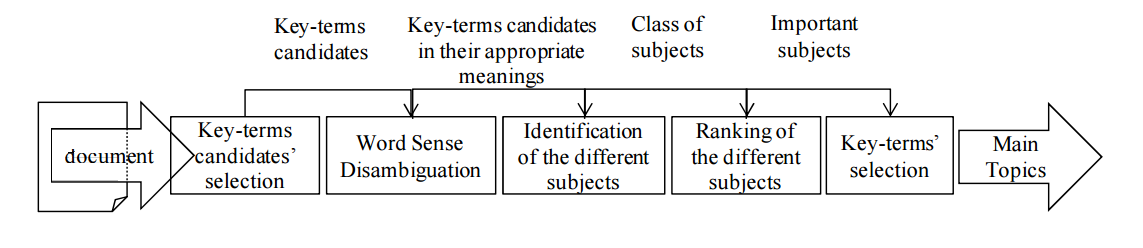
\includegraphics[scale=0.5]{topics}
\caption{The process of main topics identification }
\label{fig_topics}
\end{figure}

Among the topics found, we determine only one that will be representing the context of the document. The process of the context identification is described as follows: \\ 
We, first, calculate the similarity between all pairs of main topics by applying the similarity of Jiang and Conrath \cite{jiang}. The term which has the highest similarity rate with all the other identified main topics, is chosen as the most important topic of the document. \\

Once the most important topic of the document is identified, some additional information may be necessary. For instance, if we consider that the important topic is “Baccalaureate of 2017", the necessary additional information needed is the country where the academic qualification will be held. For example, the sentence “Tunisian Baccalaureate exams of 2017” represents a complex nominal group. In order to obtain the necessary additional information, we need to identify the different complex nominal groups in the document. A complex nominal group is a simple nominal group modified by one or two prepositional phrases.


\subsection{Extraction of significant variable data}
\label{extract_lab}
The process of extracting significant variable data \cite{maha} can be categorized in three main steps:
The first step employs the different named entities extracted in data processing stage in order to group the ones that belong to the same category (the names of persons, organizations, etc.) in a “class of category”. If we consider the following paragraph: 
“The French presidential election will be held on April 2017. The voters will go to the polls to pick their new president. Until now, the candidate, which has the highest scores of vote is Marine le Pen. This candidate credited with 27\%  of voting intention during the period of time 2-4 Mars, 2017. She obtained also 28\% during the period of time 14-16 Mars, 2017.”  
We can obtain four classes of category using the natural language processing techniques: “PERSON” that refer to a name of person, “DURATION” to a period of time, “DATE” to a given date and “PERCENT” to a percentage as shown in figure \ref{class_cat}.  

\begin{table}[H]
\centering
\caption{Different classes of categories}
\label{class_cat}
\begin{tabular}{|c|c|c|c|c|c|c|}
\cline{1-1} \cline{3-3} \cline{5-5} \cline{7-7}
\cellcolor[HTML]{FFFFFF}{\color[HTML]{333333} PERSON} &  & DURATION                                                                     &  & PERCENT                                             &  & DATE       \\ \cline{1-1} \cline{3-3} \cline{5-5} \cline{7-7} 
Marine le Pen                                         &  & \begin{tabular}[c]{@{}c@{}}14-16 Mars, 2017\\ 2-4 Mars, 2017\end{tabular} &  & \begin{tabular}[c]{@{}c@{}}27\%\\ 28\%\end{tabular} &  & April 2017 \\ \cline{1-1} \cline{3-3} \cline{5-5} \cline{7-7} 
\end{tabular}
\end{table}

Once the different classes of categories are extracted, the problem arises in entities of a same category that may belong to different concepts. Therefore, we need to gather the different named entities that belong to the same concept as a single entity called “class of concepts”. Considering the class of category “PERSON” that contains different names of candidates and voters as described in table \ref{class_of}.


\begin{table}[H]
\centering
\caption{Class of category}
\label{class_of}
\begin{tabular}{|c|}
\hline
Person                                                                                                   \\ \hline
\begin{tabular}[c]{@{}l@{}}Marine le Pen\\ François Fillon\\ Fabien Martin\\ Marcel Laurent\end{tabular} \\ \hline
\end{tabular}
\end{table}

In this case, the process must be able to differentiate between both concepts \textit{“candidate” and “voter”}. Using the \textif{“Ontology of the Context"}, we notice that \textit{“Marine Le Pen”} and \textit{“François Fillon”} belong to the concept \textit{“candidate”} while \textit{“Fabien Martin”} and \textif{“Marcel Laurent”} are unknown persons. Therefore, the classification will be based on belonging to the same concept and thus allowing us to obtain the following classes of concepts presented in table \ref{Different_class}.

\begin{table}[H]
\centering
\caption{Different classes of concepts}
\label{Different_class}
\begin{tabular}{|c|c|c|}
\cline{1-1} \cline{3-3}
Candidate                                                                &  & Unknown person                                                         \\ \cline{1-1} \cline{3-3} 
\begin{tabular}[c]{@{}l@{}}Marine le Pen \\ François Fillon\end{tabular} &  & \begin{tabular}[c]{@{}l@{}}Fabien Martin\\ Marcel Laurent\end{tabular} \\ \cline{1-1} \cline{3-3} 
\end{tabular}
\end{table}

After identifying the different classes of concepts, we move to the detection of variables step. Therefore, we need to identify the possible relationships between each couple of classes. To do this, some algorithms have been developed in  in order to extract the different variables and store them in a structured sheet format similar to the one presented in the. These algorithms aims to build a matrix M with n rows (representing the number of sentences of the document) and three columns representing respectively nouns, verbs and complements, that will be extracted from each sentence. Then, splits up the matrix M into several sub-matrices (Mk) based on synonyms verbs. Finally, identifies the variables that can be plot graphically.
The output of the extraction of variable data process after processing is the following table \ref{different_var}: 


\begin{table}[]
\centering
\caption{Different variables extracted}
\label{different_var}
\begin{tabular}{|c|c|c|}
\hline
Candidate                                                           & Duration                                                                  & Percent                                             \\ \hline
\begin{tabular}[c]{@{}c@{}}Marin le Pen\\ Marin le Pen\end{tabular} & \begin{tabular}[c]{@{}c@{}}2-4 Mars, 2017\\ 14-16 Mars, 2017\end{tabular} & \begin{tabular}[c]{@{}c@{}}27\%\\ 28\%\end{tabular} \\ \hline
\end{tabular}
\end{table}


\subsection{Relationship extraction}
\label{sec_22}

%%The process of automatic detection of variables will differentiate between categories of these variables and the different models of graphical representations. In this step, we need information concerning the graphical representation model and the variable data extracted from a given document. This process will be implemented using various NLP techniques.
Relation Extraction (RE) \cite{reeeeeeee} consists of the identification of the semantic relations between pairs of terms in unstructured or semi-structured natural language documents. Semantic relations are useful for several applications, including the acquisition of terminological data, construction and extension of lexical resources and ontologies, question answering, information retrieval, semantic web annotation, etc. In our proposed approach here, some existing text processing tools should be able to extract the relations between the variable data instances. The approach is consisted of mapping linguistic components with some syntactic relationship (a linguistic triple) and the mapping between terms and concepts is guided by a domain ontology and a named entity recognition system. A linguistic triple can contains three terms: A subject, a property and an object. E.g: A raw text containing the sentence "The lion belongs to the carnivores species." , the linguistic triple that should be extracted is: 
"lion" as the subject, "belong\_to" as the property and "carnivores" as the object. 



\section{Ontology Construction}

%%\section{Applied Ontologies}
\label{sec_3}
We use two ontologies in our proposed approach - the first one is the Ontology of the context generated after the detection of the the main topics, the context and the variable data, and secondly, the Graphical representation Ontology that is created manually. 
%%but in this step we will only focus on the automatic construction of the "Ontology of the context". 

\subsection{Ontology of the Context}
\label{sec_33}
Before jumping up and creating the context ontology, we must first look for other existing ontologies out there on the Internet using Ontology search engines like OntoSearch \cite{ontosearch}. If the context already exists, we will be using and populating it with our variable data and relations found retrieved from our analyzed document. And if the Ontology of the corresponding context is not found, we will proceed and create a new ontology related to the new context found.  
%%\begin{figure}[H]
%%\centering
%%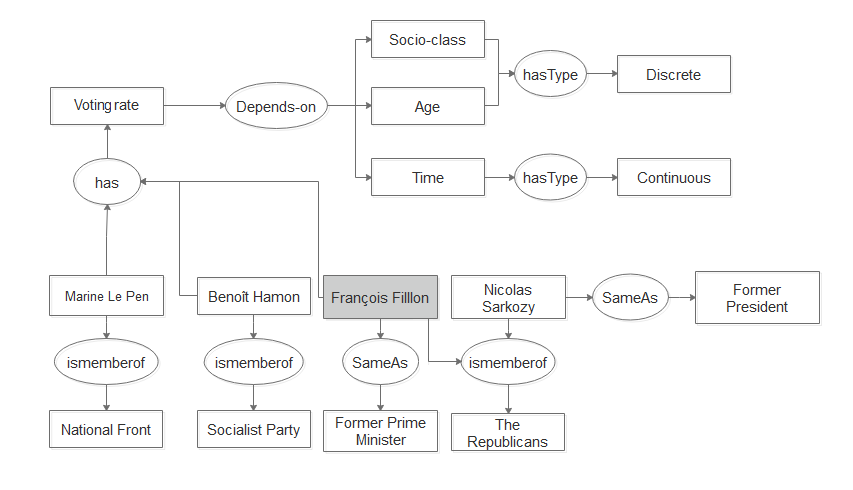
\includegraphics[scale=0.7]{contextOnt}
%%\caption{An example of a Context ontology}
%%\label{fig_context}
%%\end{figure}

\subsection{Ontology of the Graphical models}
\label{sec_44}
Generally, graphical models are those that were introduced by William Playfair where  he invented three of the four basic forms of graph: the statistical line graph, the bar graph and the pie graph. In 1786 he published “Commercial and Political Atlas” \cite{graphmodel} that contained 44 graphs. Modern statistical graphs are almost identical to those published by Playfair.

A Bar graph \cite{graphmodel} is drawn through columns of equal width and different heights. Three Types of Bar graphs are used to represent different data sets: The simple bar diagram, Compound bar diagram and Polybar diagram. The figure \ref{fig_bar} present a compound graph.

\begin{figure}[H]
\centering
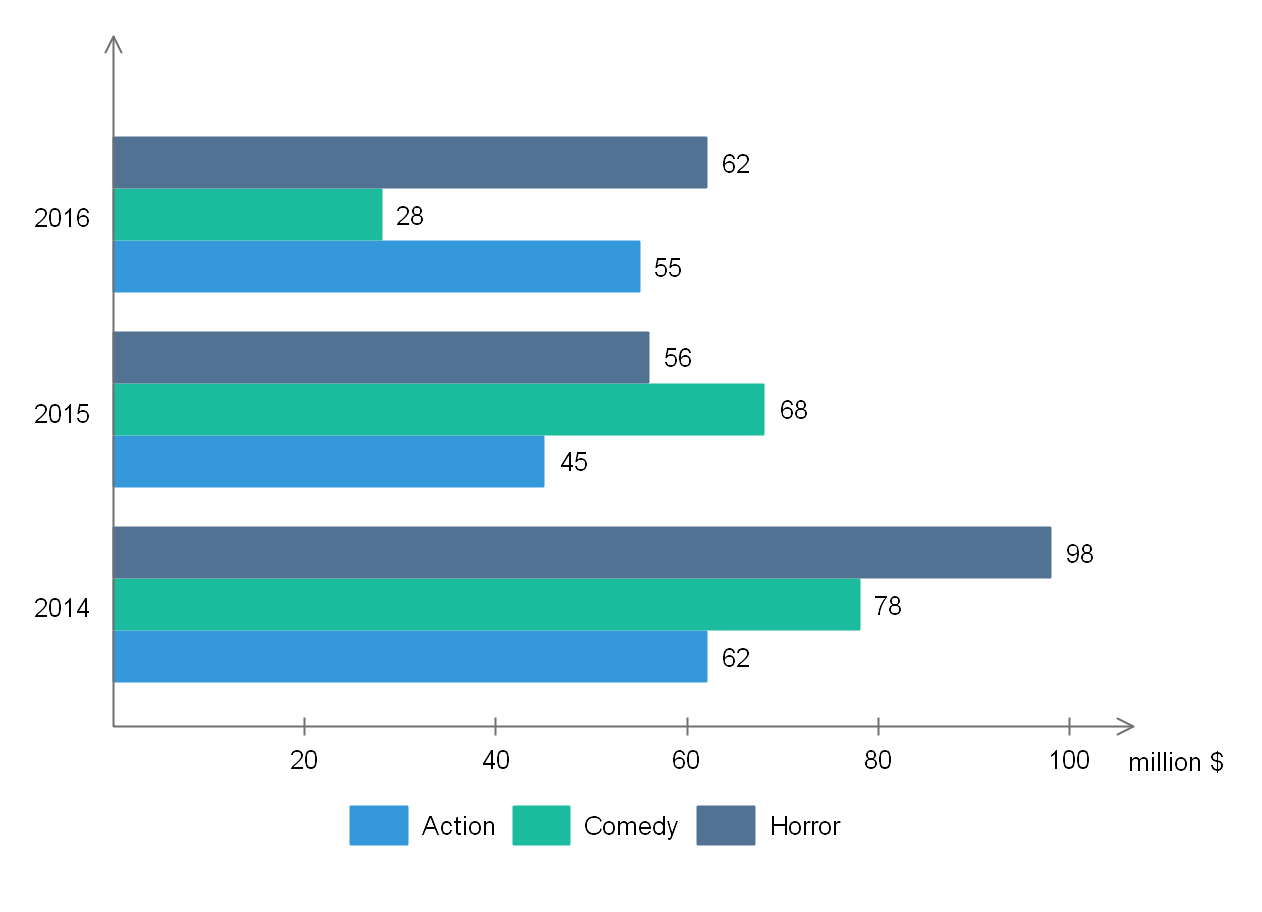
\includegraphics[scale=0.4]{compound}
\caption{Compound diagram of movie sales growth}
\label{fig_bar}
\end{figure}

A Pie diagram \cite{graphmodel} as presented in the figure \ref{fig_pie} is drawn to represent the total value of the given attribute using a circle. Dividing the circle into corresponding degrees of angle then represent the subsets of the data. Hence, it is also called as Divided Circle Diagram.


\begin{figure}[H]
\centering
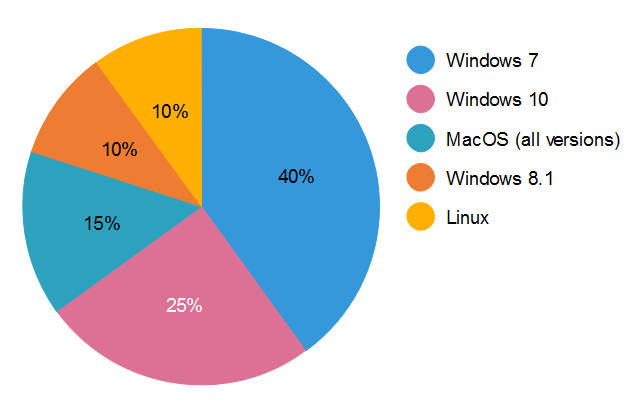
\includegraphics[scale=0.5]{piechart}
\caption{Pie diagram of operating systems usage}
\label{fig_pie}
\end{figure}
\newpage

The Line graphs \cite{graphmodel} as presented in the figure \ref{fig_poly} are usually drawn to represent the time series data. Example: temperature, rainfall, population growth, birth rates and the death rates, unemployment rates.

\begin{figure}[H]
\centering
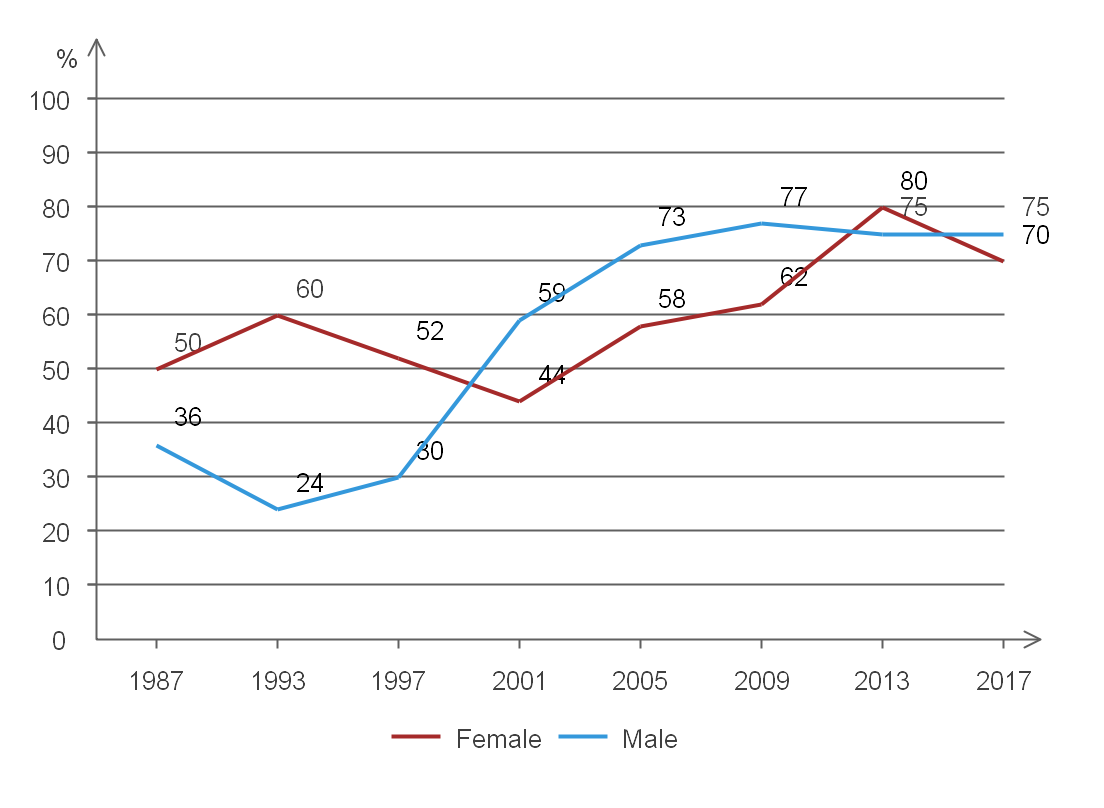
\includegraphics[scale=0.5]{linegraph}
\caption{Polygraph of unemployment rates}
\label{fig_poly}
\end{figure}


According to our proposed approach, we create a static and unique Ontology that is used each time the problem of the graphical representation on demand arises. The models are always the same whatever the data is about. Our idea is to refer to these models in the “Ontology of the Graphical Models” \cite{nour}.



\bigskip

\begin{figure}[H]
\centering
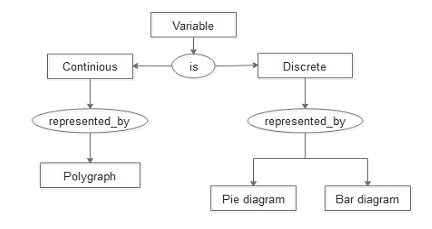
\includegraphics{Graphical_ontology}
\caption{Graphical models ontology }
\label{fig_Graphical_ontology}
\end{figure}


\section{Annotating the document}
\label{sec_55}

The primary purpose of annotating documents is to avoid reprocessing a document that has already been processed. A document can of course be processed several times in different contexts, but for a given context, it is a matter of "marking variable data", specifying which variable is considered as the “Principal Variable” and the others according to which this main variable varies. The annotation process is based on RDF and is deeply linked to the considered "Ontology of the Context". 




\section{On demand graphical representation}
\label{sec_66}

The on demand graphical representation relates to documents that have been already annotated. It is a fairly simple process that consists in applying the following steps:

\begin{enumerate}[label=(\alph*)]
\item Determining the variable to be represented in the y-axis. It is obtained from the overall context of the document. For example, if the context is "International Collegiate Programming Contest 2017" then the variable is the rate of solved problems. In this case the y-axis represents one or more teams for the contest.

\item  Determining the variable data to be represented in the x-axis. In our example ("International Collegiate Programming Contest 2017") can be measured according several criteria: time to represent its evolution, by duration, attempts , etc. \\
Each variable data has its own criteria which can be either discrete or continuous according to the Ontology of the "graphical models". This process of choosing criteria will be accomplished manually.
\item Retrieving the representation values from the extracted variable data instances of the current analyzed document, which guarantees that the graph is corresponding to the actual data of the context.
\item Granting the user the ability to select which graphical representation to be visualized regarding the obtained variable data and the criteria found by offering the ability to select which variable data to be shown in the x-axis and which available graphical representation to be visualized.
\end{enumerate}

 
\section*{Conclusion}


Semantic annotations describe the content of documents based on the concepts and relationships represented in an Ontology. In this context, Ontologies play an important role: they show the vocabulary and the knowledge of the field studied. These will be used to analyze the content of unstructured Web documents. The semantic annotation based on Ontology requires that it should be rich: it must represent not only the concepts and relations mentioned in the documents, but also the terms accompanied by their variants which in turn are used to denote these entities in the text.